\documentclass[class=report, float=false, crop=false]{standalone}
% \usepackage[subpreambles=true]{standalone}

%%%% PACKAGES

\usepackage{import}
\usepackage[toc,page]{appendix}
\usepackage[T1]{fontenc}
\usepackage[english]{babel}
\usepackage[utf8]{inputenc} 
\usepackage{graphicx}
\usepackage{adjmulticol}
\usepackage[labelfont=bf]{caption}
\usepackage{graphicx}
\usepackage{subcaption}
\usepackage{fancyhdr}
\usepackage{url}
\usepackage{amsmath} % collection de symboles mathématiques
\usepackage{amssymb} % collection de symboles mathématiques
\usepackage{amsthm}
\usepackage{bbm}
\usepackage{bm}
\usepackage{stmaryrd}
\usepackage{mathtools}
\usepackage{cancel}
\usepackage{titling}
\usepackage{nameref} % pour désigner des parties par leur nom
\usepackage{url} % pour mettre des URL
\usepackage{cite}
% \usepackage[sectionbib]{chapterbib}
% \usepackage{chapterbib}
\usepackage[numbers,sort&compress]{natbib}
% \usepackage[square,numbers,sectionbib]{natbib}
% \usepackage{bibunits}
% \usepackage{biblatex}
\usepackage{tabularx}
\usepackage{titlesec, blindtext, color}
% \usepackage{auto-pst-pdf}

%%%% TIKZ

\usepackage{pgf, tikz}
\usetikzlibrary{shapes.misc}
\usetikzlibrary{decorations.pathreplacing}

\tikzset{cross/.style={cross out, draw=black, minimum size=2*(#1-\pgflinewidth), inner sep=0pt, outer sep=0pt},
%default radius will be 1pt. 
cross/.default={0.25pt},
    point/.style={
    thick,
    draw=black,
    cross out,
    inner sep=0pt,
    minimum width=4pt,
    minimum height=4pt,
    },
}

%%%% STYLE

% \textheight=21 true cm
% \textwidth= 15. true cm
% \oddsidemargin=0.5truecm
% \evensidemargin=0.5truecm
% \topmargin=0.1truecm

% \setlength{\topmargin}{-1cm}
\setlength{\headheight}{0.43cm}
\setlength{\headsep}{0.8cm}
\setlength{\footskip}{0cm}
\setlength{\textwidth}{17cm}
\setlength{\textheight}{23.5cm}
\setlength{\voffset}{-2.5cm}
\setlength{\hoffset}{-0.25cm}
\setlength{\oddsidemargin}{0cm}
\setlength{\evensidemargin}{0cm}
\setlength{\parindent}{0pt}
\setlength{\footskip}{30pt}

\setlength{\droptitle}{-6cm}

\setcounter{tocdepth}{3}
\setcounter{secnumdepth}{3}

\definecolor{lcolor}{rgb}{0,0,0.6} % définition de la couleur des liens pdf
\usepackage{hyperref}
\hypersetup{pdftex,colorlinks=true,
linkcolor=lcolor,
citecolor=lcolor,
urlcolor=lcolor,
hyperindex=true,
hyperfigures=false} % fichiers pdf 'intelligents', avec des liens entre les références, etc.

\definecolor{gray75}{gray}{0.75}

\AtBeginDocument{\addtocontents{toc}{\protect\thispagestyle{empty}}}

% \titleformat{\chapter}[hang]{\vspace{-50pt}\huge\bfseries}{\thechapter\hspace{20pt}\textcolor{gray75}{|}\hspace{20pt}}{0pt}{\huge\bfseries}
\titleformat{\subsection}[block]{\hspace{2em}}{\large\textbf\thesubsection}{1em}{\large\textbf}
\titleformat{\subsubsection}[block]{\hspace{4em}}{\small\textbf\thesubsubsection}{1em}{\small\textbf}

\usepackage{etoolbox}
\makeatletter
\patchcmd{\@chap@pppage}{\thispagestyle{plain}}{\thispagestyle{empty}}{}{}
\makeatother

\captionsetup{font=normalsize}
\captionsetup[sub]{font=scriptsize}

%%%% COMMANDS

%\renewcommand*\thesection{\arabic{section}}

\makeatletter
\providecommand*\bigcdot{\mathpalette\bigcdot@{.5}}
\providecommand*\bigcdot@[2]{\mathbin{\vcenter{\hbox{\scalebox{#2}{$\m@th#1\bullet$}}}}}
\makeatother

\providecommand{\appropto}{\mathrel{\vcenter{
  \offinterlineskip\halign{\hfil$##$\cr
    \propto\cr\noalign{\kern2pt}\sim\cr\noalign{\kern-2pt}}}}}

\providecommand\encircle[1]{%
  \tikz[baseline=(X.base)] 
    \node (X) [draw, shape=circle, inner sep=0] {\strut #1};}

\providecommand\phantomarrow[2]{%
  \setbox0=\hbox{$\displaystyle #1\to$}%
  \hbox to \wd0{%
    $#2\mapstochar
     \cleaders\hbox{$\mkern-1mu\relbar\mkern-3mu$}\hfill
     \mkern-7mu\rightarrow$}%
  \,}

\providecommand{\myparagraph}[1]{\paragraph{#1}\mbox{}\\\vspace{-5pt}}

\providecommand{\isEquivTo}[1]{\underset{#1}{\sim}}

\makeatletter
\providecommand{\subalign}[1]{%
  \vcenter{%
    \Let@ \restore@math@cr \default@tag
    \baselineskip\fontdimen10 \scriptfont\tw@
    \advance\baselineskip\fontdimen12 \scriptfont\tw@
    \lineskip\thr@@\fontdimen8 \scriptfont\thr@@
    \lineskiplimit\lineskip
    \ialign{\hfil$\m@th\scriptstyle##$&$\m@th\scriptstyle{}##$\crcr
      #1\crcr
    }%
  }
}
\makeatother

% \makeatletter
% % Original \l@section:
% %\renewcommand*\l@section{\vskip 6pt plus 1pt minus 1pt
% %                         \@dottedtocline{1}{1.5em}{2.3em}}
% % Modified \l@section:
% \renewcommand*\l@section{\ifnum\c@tocdepth>\z@\vskip 6pt plus 1pt minus 1pt \fi
%                          \@dottedtocline{1}{1.5em}{2.3em}}
% \makeatother

\providecommand\smallO[1]{
      \mathchoice
         {% mode \displaystyle
            \ensuremath{\mathop{}\mathopen{}{\scriptstyle\mathcal{O}}\mathopen{}\left(#1\right)}
         }
         {% mode \textstyle
            \ensuremath{\mathop{}\mathopen{}{\scriptstyle\mathcal{O}}\mathopen{}\left(#1\right)}
         }
         {% mode \scriptstyle
            \ensuremath{\mathop{}\mathopen{}{\scriptscriptstyle\mathcal{O}}\mathopen{}\left(#1\right)}
         }
         {% mode \scriptscriptstyle
            \ensuremath{\mathop{}\mathopen{}{o}\mathopen{}\left(#1\right)}
         }
   }

%%%% PATCH

% \makeatletter
% \let\orig@document\document
% \let\orig@enddocument\enddocument
% \def\sa@document{%
%   \endgroup
%   \global\let\enddocument\sa@enddocument
%   \sa@atbegindocument
% }
% \def\sa@enddocument{%
%   \sa@atenddocument
%   \global\let\document\orig@document
%   \global\let\enddocument\orig@enddocument
%   \begingroup
%   \@ignoretrue
%   \def\@currenvir{document}%
%   \aftergroup\endinput
% }
% \makeatother

\graphicspath{ {.} }

\begin{document}

\thispagestyle{empty}


\includegraphics[height=2cm]{logoens.eps} \hfill 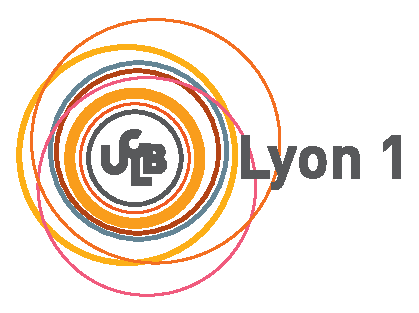
\includegraphics[height=2cm]{logoucbl.eps} \hfill 
\includegraphics[height=2.5cm]{udl-logo.png}

\vspace{0.5cm}

\begin{tabularx}{\textwidth}{ @{} l X r @{} }
{\sc Master Sciences de la Matière} & & Phase Transitions and Critical Phenomena \\
{\it École normale supérieure de Lyon} & & \textbf{Yann-Edwin KETA} \\
{\it Université Claude Bernard Lyon 1} & & M2 Physique -- 2017-2018
\end{tabularx}

\begin{center}

%\rule[11pt]{17cm}{0.5pt}


\vspace{1.5cm}

\textbf{\huge Nematic order in packings of spheroids}


%\rule{12cm}{2pt}

\vspace{2cm}

\parbox{12cm}{\small
\textbf{Abstract}: \it We first give evidence of a density-driven isotropic-nematic transition of first order in static packings of hard-core spheroids, based on results derived from recent theoretical developments by Nascimento et al. We then investigate the effect of the jamming transition on the orientational order in sheared packings of soft-core spheroids based on numerical simulations.
%We present here the methods and models we have developed or adapted from the study of static or sheared packings of spheres to the study of sheared packings of spheroids. These allow us to investigate the critical behaviours observed at the jamming transition and the other behaviours observed near the rheological transition of packings of soft-core frictionless spheroids. We show that our models give results in good accordance with existing literature and point out interesting phenomena which could give new insights into the jamming transition.
} %fin de la commande \parbox du résumé


\vspace{0.5cm}

% \parbox{15cm}{
% \textbf{Keywords}: \it .
% } %fin de la commande \parbox des mots clefs

\vspace{5cm}


\includegraphics[height=4cm]{SdM.png}

\end{center}

\vfill
\newpage

\end{document}